\chapter{RDF data generation from non-RDF data}
\label{chap:rdf_data_generation}

How do we generate RDF data from non-RDF data? A variety of specifications and languages exists
which define the generation of RDF data from non-RDF data. These specifications and languages can be grouped 
into two major groups; query languages and mapping languages. Several state-of-the art implementations, 
utilizing these two groups of languages, exist to generate RDF data from non-RDF data.

The implementations can be categorized into two groups; \emph{query-based} and 
\emph{rule-based} implementations. These can be further categorized into two more subgroups 
based on the data that they consume; \emph{bounded} and \emph{unbounded} data. 
This work will focus on 
implementations working with unbounded data in a streaming environment (Chapter~\ref{chap:intro}), 
thus implementations 
consuming bounded data will not be elaborated. 
In this section, we will first discuss the \emph{languages} these implementations employ 
to transform non-RDF to RDF data. Finally, the details of the implementations are elaborated 
with simple examples. 


\section{SPARQL Query Language}
Query languages such as SQL~\cite{sql} already exist in established relational database systems such as 
MySQL or PostgreSQL. It allows users to manipulate and retrieve data 
from relational databases using concise statements. Due to its widespread 
use in the industry for querying databases, it is important that a similar 
query language is used for RDF datasets to ease the transition for the users. 

SPARQL~\cite{sparql} achieves this goal by having SQL-like syntax to allow 
a seamless transition to RDF for existing data engineers. 
In terms of relational databases, RDF 
datasets can be viewed as a table consisting of three columns --- the \textit{subject} column, 
the \textit{predicate} column, and the \textit{object} column. Unlike relational databases, 
RDF datasets, in a table representation, allow the object column to be of heterogeneous 
datatype~\ref{sec:turtle_syntax}. 


Moreover, different from SQL, SPARQL allows matching based on \emph{basic graph patterns} composed 
of a set of \emph{triple patterns}. Triple patterns are similar to the triple statements 
as clarified in Section~\ref{sec:turtle_syntax} but extended with declared variables (i.e. \emph{?variable\_name}). 
The declared variables are then bound to the concrete value in the corresponding \emph{triple statements},
matching the given \emph{triple pattern}, from the RDF dataset. 
The result of a SPARQL query is returned as an RDF sub-graph of the queried RDF dataset. 

How does this query language relate to transforming an 
unbounded dataset to RDF format in a streaming environment? There exists state-of-the-art 
engines utilizing SPARQL syntax for generating RDF data from heterogeneous streaming data sources, which will be 
elaborated in Section~\ref{sec:query_based_implementations}. 

\begin{lstlisting}[language=SPARQL,
    caption={Example of a SPARQL query of a medication on the given input.}, 
    label={lst:sparql_example}]
    SELECT ?medication
    WHERE {
        #Basic graph pattern consisting of 2 triple patterns. 
        ?diagnosisId example:name "Cancer" .
        ?medication example:canTreat ?diagnosisId .
    }
    ...
    ---------
    #Input RDF graph
    <http://example/diagnosisID/1> example:name "Cancer". 
    <http://example/medication/RadiationTherapy> 
            example:canTreat <http://example/diagnosisID/1>.
\end{lstlisting}
\begin{table}[!htbp]
    \centering
    \begin{tabular}{|c|}
    \hline
    \textbf{medication}        \\ \hline
    http://example/medication/RadiationTherapy\\ \hline
    \end{tabular}
    \caption{Result of executing the SPARQL query in Listing~\ref{lst:sparql_example}}
    \label{tab:sparql_result}
\end{table}


\section{RDF Mapping Language}
RDF Mapping Language~\cite{rml} is a superset of the W3C's R2RML~\cite{r2rml} which maps relational databases to
RDF datasets. RML improves upon R2RML by expressing mapping rules from heterogeneous
data sources and transforming them to RDF datasets whereas R2RML could only consume
data from relational databases. An RML mapping document is composed of one or more \emph{triples maps}, 
which in turn consist of \emph{subject, predicate} and \emph{object} term maps. As the names imply, 
the term maps are used to map elements of the data sources to their respective terms 
in an RDF triple. The definitions of these maps are similar to the 
specifications in R2RML~\cite{rml_tech}. 

Logical sources could be defined by specifying the \emph{source, logical iterator} 
and zero or one \emph{reference formulation} property.
Although the reference implementation RMLMapper could only process logical sources 
consisting of bounded data, the expressiveness and the flexibility of RML allows one 
to extend it to support unbounded data sources. For example, RMLStreamer~\cite{rml_streamer} implementation in 
Section~\ref{sec:rml_streamer} extended the base RML vocabulary to support logical sources with unbounded data. 

RML also supports defining relationships amongst the different 
triples maps through the use of \textit{rr:parentTriplesMap, rr:joinCondition, rr:child and rr:parent}
properties. Different triples maps might come from separate logical sources, therefore, 
referencing across triples maps might require applying the join operator across multiple 
logical sources. 

Moreover, an ontology to semantically define functions, FnO~\cite{fno_ben}, has been supported 
in RML, allowing users to apply user defined functions during the mapping process. This 
extension provides RML implementations with the capabilities to transform the input data with 
lightweight computations before mapping them into RDF triples; providing some form of 
data processing. 

\begin{lstlisting}[caption={An example of an RML mapping document~\cite{rml_tech}}.]
@prefix rr: <http://www.w3.org/ns/r2rml#>.
@prefix rml: <http://semweb.mmlab.be/ns/rml#>.
@prefix ex: <http://example.com/ns#>.
@prefix ql: <http://semweb.mmlab.be/ns/ql#>.
@prefix xsd: <http://www.w3.org/2001/XMLSchema#>.
@prefix rdfs: <http://www.w3.org/2000/01/rdf-schema#>.
@base <http://example.com/ns#>.

<#TransportMapping>
  rml:logicalSource [
    rml:source "Transport.xml" ;
    rml:iterator "/transport/bus/route/stop";
    rml:referenceFormulation ql:XPath;
  ];

  rr:subjectMap [
    rr:template
      "http://trans.example.com/stop/{@id}";
    rr:class ex:Stop
  ];

  rr:predicateObjectMap [
    rr:predicate rdfs:label;
    rr:objectMap [
      rml:reference "."
    ]
  ].
    
\end{lstlisting}

\section{Query based implementations}
\label{sec:query_based_implementations}

Intuitively, querying the data source with a 
query language is the common method to interact 
with a database. Allowing users to query the sources without explicitly 
defining the mapping semantics, hides the mapping or data transformation details from the user. 
Moreover, it eases the transition to developing applications using RDF data since the syntax is 
similar to the existing query languages leading to lower learning curve for the developers.
To the best of our knowledge, there exist two state-of-the-art 
template based implementations, using SPARQL query-like languages, for transforming 
unbounded non-RDF data to RDF data: SPARQL-Generate and RDF-Gen.
These implementations and approaches will be elaborated more in the following sections.


\subsection{SPARQL-Generate}
SPARQL-Generate~\cite{sparql_generate} was proposed as an alternative to existing methods of 
transforming non-RDF data. The language is based on an extension of SPARQL 1.1 query language, to leverage 
its expressiveness and extensibility. Furthermore, SPARQL-Generate can be implemented on top 
of any existing SPARQL query engine. The reference implementation in the paper was based on Apache Jena's 
SPARQL 1.1 engine. Due to the use of the existing SPARQL 1.1 query language, experienced knowledge engineers could use 
SPARQL-Generate to improve the generation of RDF data in their existing workflow. 

SPARQL-Generate supports the consumption of heterogeneous data sources by exposing the 
\emph{binding} and \emph{iterator functions API}. Therefore, covering a new data format or data source could be accomplished 
by implementing the corresponding \emph{binding} and \emph{iterator functions}. Currently, 
the reference implementation supports the consumption of data sources which are unbounded in a 
streaming environment or bounded datasets. 
For example, WebSocket and MQTT are currently supported in the latest version of SPARQL-Generate. 

Although there is a support for data stream processing, the paper did not go into details 
about the application of multi-stream operators like joins when involving multiple streaming 
data sources. M. Lefran\c{c}ois~\cite{sparql_generate} clarified that when joining
records from two different streams, SPARQL-Generate will fully consume the records 
from the "parent" stream and index it internally. The "child" stream will then be iteratively consumed and 
joined with the records from the internal index. Hence, we could assume that SPARQL-Generate processes the "parent" 
stream in memory when there is a multi-stream operator.
Furthermore, it is mentioned that SPARQL-Generate could use the SPARQL 1.1 operators such as \emph{join operators}. 
From this, we could derive that SPARQL-Generate will apply \emph{join} on the 
records by delegating it to the underlying SPARQL engine.
Therefore, there is a lack of  
dynamic windowing schemes to efficiently exploit the characteristics of the streaming data sources.  


\section{Mapping based implementations}
\label{sec:mapping_based_implementation}
Other than approaching the transformation of non-RDF to RDF from the viewpoint of 
queries, one could also employ mapping languages such as RML. Mapping languages 
are declarative and have minimal cognitive burden composing it compared to the
query based implementations; one does not need to deal with nested queries,
due to defining the mapping relationship for each attribute in 
the input source. Despite being more 
verbose than query languages, composing complex mapping documents results in much more human-readable 
format due to the direct mapping of the attributes. 
The following subsections will elaborate more on the related state-of-the-art engines 
which utilizes mapping languages in a streaming environment.

\subsection{TripleWave}
Albeit the abundance of solutions to combine semantic technologies with stream and event processing 
techniques, there was a lack of engines to disseminate and exchange RDF streams on the Web~\cite{triple_wave}. 
TripleWave~\cite{triple_wave} was conceived to fill this role; to provide the mechanism to publish and spread RDF streams on the Web. 
It extends R2RML, which only allows ingestion of inputs from relational databases, 
to also consume other formats such as JSON or CSV (just like RML, a superset of R2RML). 

TripleWave generates an RDF stream of JSON-LD format, which could be consumed by existing
RDF Stream Processing (RSP) engines as input, for the publication of RDF data.
It also supports joining of multiple streams which could be inferred from its implementation of R2RML's \emph{rr:parentTriplesMap} predicate~\cite{triple_wave}. Since the goal of TripleWave 
is to publish RDF streams from RDF and non-RDF data sources, it does not support the 
application of arbitrary functions at its core unlike RDF-Gen and SPARQL-Generate. 
However, as is the case with the aforementioned frameworks and engines, 
it does not support dynamic windowing to handle streams 
with dynamic characteristics. 


\begin{figure}[!htbp]
  \centering
  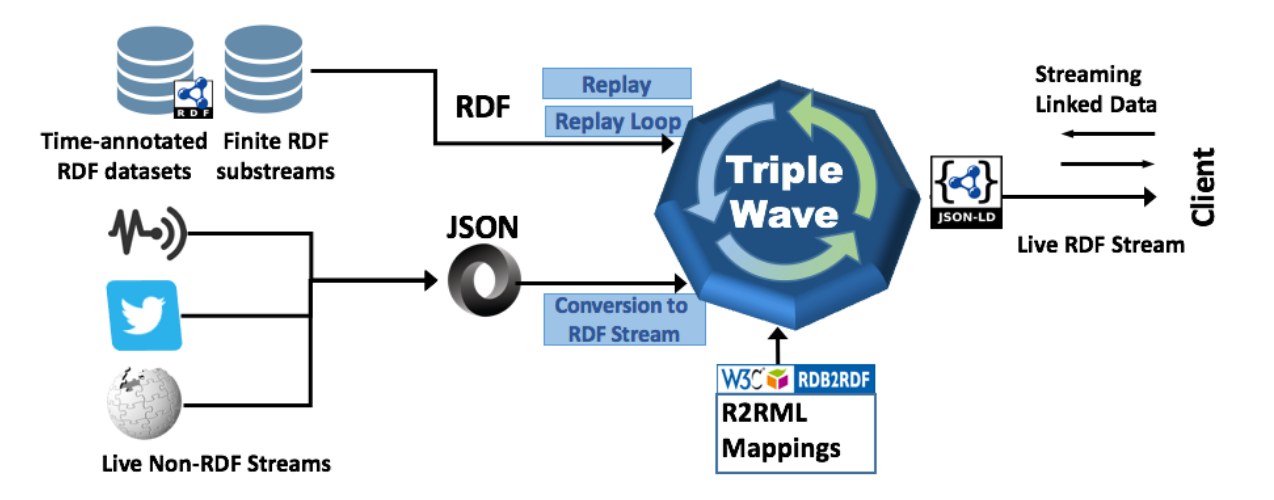
\includegraphics[width=\textwidth]{fig/triple-wave-arch.png}
  \caption{Architecture of TripleWave generating RDF streams from non-RDF and RDF data sources~\cite{triple_wave}. }
  \label{fig:triple-wave-arch}
\end{figure}

\paragraph{The shortcomings}%
The implementations elaborated thus far, scale insufficiently in terms of velocity and 
volume of data streams. Multiple instances of the engines will need to 
be started in order to scale with the higher volume and velocity of 
the input data streams. Since they are not built upon a distributed framework, 
there is also a need for a separate implementation to coordinate the different 
instances in a distributed environment. 

\subsection{RMLStreamer}
\label{sec:rml_streamer}
RMLStreamer~\cite{rml_streamer}
was developed to parallelize the ingestion and mapping process of RDF data generation pipeline. 
It is based on the work of RMLMapper~\cite{rml}, an RDF mapping engine consuming bounded data and 
mapping them to RDF data with the use of RML. Hence, RMLStreamer can also 
process heterogeneous data and generate RDF data. 

Due to the parallelization of the subtasks, the ingestion and the mapping process, these processes
could be spread over different machines for distributed execution (Figure \ref{fig:rml-parallel-arch}). 
However, a mechanism to coordinate the different machines is required in the environment of 
distributed computing.  
To fulfill this requirement, RMLStreamer is 
implemented on top of Apache Flink~\cite{flink} framework (Section \ref{sub:Apache Flink}). Not only does it allow the mapping 
of non-RDF to RDF data, it also guarantees fault-tolerance through the usage of 
\emph{Asynchronous Barrier Snapshots}~\cite{flink_fault_tolerance} and \emph{exactly-once} semantic,
although these are disabled by default. 

\begin{figure}[!htbp]
  \centering
  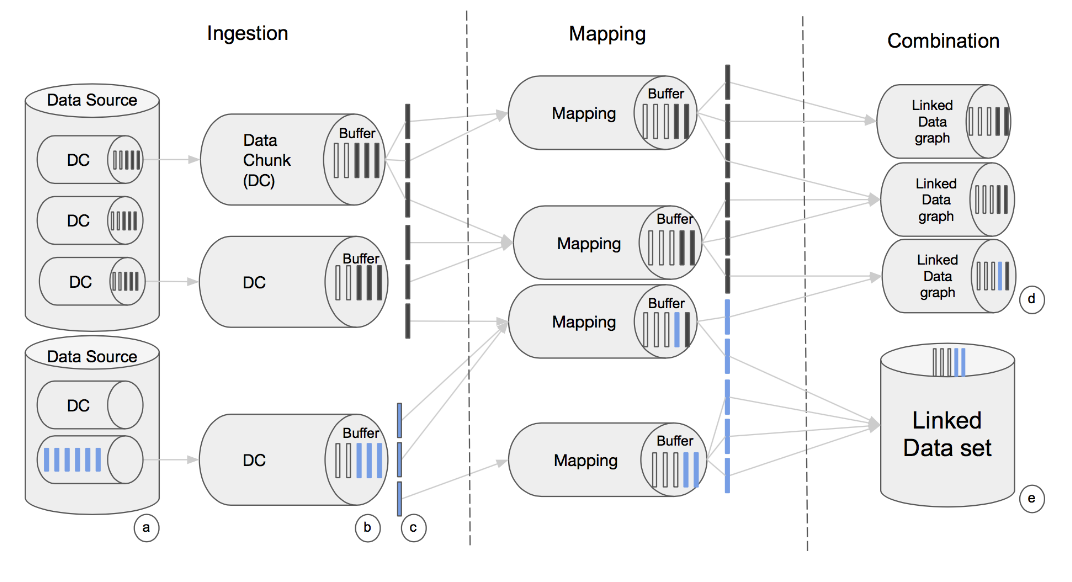
\includegraphics[width=\textwidth]{fig/rml_streamer_arch.png}
  \caption{Parallelization architecture of RMLStreamer for RDF data generation~\cite{rml_streamer}. RMLStreamer parallelizes 
  the ingestion of the data sources and the mapping process of non-RDF to RDF data. }
  \label{fig:rml-parallel-arch}
\end{figure}



\section{Custom syntax implementation}
Unlike the aforementioned two categories of implementations based on one of the
standardized syntaxes, 
there exists implementations which combines pieces of both. RDF-Gen is one such 
implementation with its own custom syntax. 

\subsection{RDF-Gen}
RDF-Gen~\cite{rdf_gen} is based on its own custom syntax 
similar to a combination SPARQL and Turtle syntax. 
Unlike SPARQL-Generate, instead of extending SPARQL engines, 
it provides its own architecture to meet the demands
of real-time processing (Figure~\ref{fig:rdf-gen-arch}). 
Through combination of SPARQL and Turtle syntax, RDF-Gen 
keeps the basic graph pattern section of SPARQL query with 
the specifications of term nodes from Turtle to reduce
the size of the transformation specification.  

RDF-Gen consists of three main components: 
\begin{enumerate*}[label=(\alph*)]
  \item Data Connector,
  \item Triple Generator, and
  \item Link Discovery.
\end{enumerate*}

Data Connectors allows close-to-source processing. This is due to the
data consumption 
module being decoupled from the mapping process as shown in Figure ~\ref{fig:rdf-gen-arch}. 
Triple Generator handles the rapid generation of RDF triples by making use of 
template graphs and variable vectors. The Link Discovery component solves the 
problem of link discovery which is defined as follows:

\begin{defn}[Link Discovery problem]    
Given two data sources $S$ and $T$, the link discovery problem is to
find the pairs of elements in 
$S \times T$ that are related to each other (e.g. following the predicate of 
\emph{owl:sameAs} property). 
\end{defn}

Link discovery remains out of scope of this thesis as we mainly focus on 
multi stream operators during RDF generation.

\begin{figure}[!htbp]
  \centering
  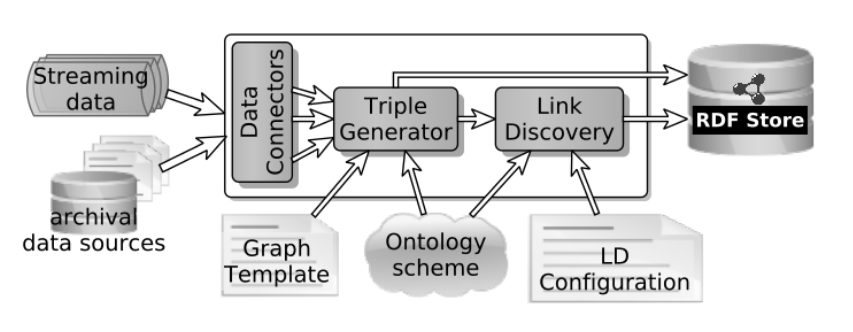
\includegraphics[width=0.8\textwidth]{fig/rdf-gen-arch.png}
  \caption{Architecture of RDF-Gen with dataflow from input sources, and 
  components requiring their specific configuration files~\cite{rdf_gen}}
  \label{fig:rdf-gen-arch}
\end{figure}

\subsubsection{Data Connector}
Data Connector has a similar functionality as the \emph{iterator functions} from SPARQL-Generate.
It consumes the data sources given a configuration setting. The configuration setting is used to specify 
the type of data sources, the \emph{window} for processing the incoming data records and 
also apply functions on the incoming data elements. Data Connector can thus be defined as a 
mapping function as in Definition~\ref{defn:data_connector}. 


\begin{defn}[Data Connector record~\cite{rdf_gen}]
  \label{defn:data_connector}
  Given a set of data sources $D = \{d_1, d_2, \dots, d_n\}$ and  a 
  mapping function $F = \mu_{f}(d_i, e)\; |\; \forall d_i \in D$ with $e$, a data element 
  of a data source $d_i$, and $f$, a filter function. Data Connector 
  generates a record $R = \mu_{f}(d_i, e)$ $\iff$ all the attributes of 
  $e$ satisfy the filter function $f$. By default, the filter function $f$ just returns true. 
\end{defn}

Using the Definition~\ref{defn:data_connector}, we could now also apply an equi-join operator 
on the data sources. Formally, we could generate a new triple 
$R =  \mu_{f_i}(d_i, e_i) \bowtie  \mu_{f_j}(d_j, e_j) $ where $e_i$ and $e_j$ have 
common attributes under the filter functions $f_i$ and $f_j$. 

The processing is done on individual records, leading to 
RDF-Gen treating streaming and archival data sources the same way --- as “streams” 
of records. Due to the record-by-record processing, the framework also has a very low 
memory usage. 

\subsubsection{Triple Generator}
Triple Generator consumes the output records 
of the Data Connectors to convert them into RDF triples (Figure~\ref{fig:rdf-gen-arch}). A vector of variables $V$, an RDF 
graph template $G$, akin to the basic graph pattern from SPARQL 1.1, and a 
set of \emph{functions} $F$ can be used to configure the Triple Generators. 

$V$ consists of variables which corresponds to the attributes of the
generated records from the Data Connector. These variables are referenced 
in the graph template $G$, and then used to 
bind to the attribute value of the record provided by the Data Connector. 
In case these variables are the arguments of a function $f \in F$, the function will 
be evaluated and the result appended to the output. Therefore, 
this simple binding of values in a template graph enables Triple Generator to 
generate RDF triples efficiently and have a high scalability.
The functions will have to be simple in complexity to keep the computation 
time as low as possible.


In this paragraph, we will illustrate how a Triple Generator works
in practice through an example.  
Listing~\ref{lst:rdf_gen_example} shows an example of a graph template $G$ provided to 
the Triple Generator to generate RDF triples. In this example, the provided vector 
of variables is $V = [\textrm{?diagnosis\_id}, \textrm{?name} ]$. Using the record 
from Table~\ref{tab:rdf_gen_sample_record}, the specified variables,
\emph{diagnosis\_id} and \emph{name}, will be bound to the values \emph{100} and 
\emph{Cancer} respectively. Afterwards, the functions \emph{makeUri} and \emph{asString} will 
be called with the bounded values as arguments and the generated 
output will be used to generate the RDF triples specified by 
the graph template. 
The final generated set of RDF triples is (e.g. in Turtle format): 

\begin{lstlisting}
  ... 
  <http://example.com/100>  a example; 
                            example:name  "Cancer". 
  ...
\end{lstlisting}


\begin{table}[!htbp]
  \centering
  \begin{tabular}{l|l}
  \multicolumn{1}{c|}{\textbf{diagnosis\_id}} & \multicolumn{1}{c}{\textbf{name}} \\ \hline
  100                                 & Cancer                    
  \end{tabular}
  \caption{A sample record generated by the Data Connector.}
  \label{tab:rdf_gen_sample_record}
  \end{table}

\begin{lstlisting}[language={SPARQL},
   caption={A simple graph template $G$ with the functions \emph{asString} and \emph{makeUri}.}, 
   label={lst:rdf_gen_example}
  ]
  #BGP for the diagnosis data source
  makeUri(?diagnosis_id)  a example:Diagnosis;
                          example:name asString(?name).
\end{lstlisting}

Consuming the input data on a record-by-record basis results in RDF-Gen having to 
handle multi-stream operators with the use of windows. However, the paper did not 
mention in detail about its implementation of windows to handle 
multi-stream operators since it was out of scope. Therefore, we still have no 
notion of how to handle data streams with dynamic characteristics where fixed windows 
size have negative consequences on the quality of the generated RDF data. 

\section{Summary}
While SPARQL-Generate~\cite{sparql_generate}, RDF-Gen~\cite{rdf_gen}, and TripleWave~\cite{triple_wave} 
support the join operator for executing a binary join, scalability is not built in those implementations
to handle multiple streaming 
data sources with high velocity and volume. 
Therefore, a solution
with built-in capabilities to handle high velocity and volume of data, is of interest
to implement the dynamic windowing scheme. 
Hence, RMLStreamer is the best candidate for this work on dynamic window in RDF generation. 
